\documentclass[11pt,a4paper]{article}

\usepackage{CJKutf8}
\usepackage{amsmath,amssymb}
\usepackage{booktabs}
\usepackage{graphicx}
\usepackage{float}
\usepackage{geometry}
\usepackage{array}
\usepackage{longtable}
\usepackage{xcolor}
\usepackage{enumitem}
\usepackage{pgfplots}

\pdfmapfile{+gbsnu.map}
\graphicspath{{report/5.6_report/}{./}}
\pgfplotsset{compat=1.18}

\geometry{left=2.4cm,right=2.4cm,top=2.3cm,bottom=2.3cm}
\setlength{\parindent}{2em}
\setlength{\parskip}{0.35em}
\setlist[itemize]{leftmargin=2em,itemsep=0.2em,topsep=0.2em}
\setlist[enumerate]{leftmargin=2em,itemsep=0.2em,topsep=0.2em}

\newcommand{\code}[1]{\texttt{#1}}
\newcommand{\figwidth}{0.92\textwidth}

\begin{document}
\begin{CJK*}{UTF8}{gbsn}

\begin{center}
  {\LARGE \textbf{\code{yolo\_final} 项目汇报辅助材料}}\\[0.8em]
  {\Large 第一部分：模型架构模块介绍}\\[0.8em]
  {\normalsize 2026 年 5 月 6 日}
\end{center}

\vspace{1em}

\section*{本部分汇报目标}

本部分用于介绍 \code{yolo\_final} 当前实验线中检测模型的核心结构。汇报重点不是泛泛介绍 YOLO，而是说明我们当前代码中实际使用的网络模块、张量流向、检测结果生成方式以及训练 loss 的组成。需要讲清楚的内容包括：

\begin{enumerate}
  \item \code{yolo\_final} 的网络架构；
  \item \code{yolo\_final} 的 backbone 结构；
  \item backbone 中使用的小模块；
  \item 检测器整体结构；
  \item decoupled head 的结构；
  \item prediction tensors 到最终 detection results 的转换；
  \item 最终训练使用的 loss 结构，以及每一个 term 的具体含义。
\end{enumerate}

当前主线实验采用 COCO-only 训练评估，输入分辨率为 $416 \times 416$，模型配置为 \code{deep\_residual\_dual\_scale\_three\_box}，使用 P4/P5 双尺度输出、每尺度 3 个 anchor、轻量 FPN/PAN neck 和 decoupled detection head。P3 是后续扩展实验方向，本部分先以当前 P4/P5 双尺度主线模型为核心对象。

\begin{table}[h]
\centering
\caption{当前主线模型配置}
\begin{tabular}{ll}
\toprule
项目 & 当前配置 \\
\midrule
输入分辨率 & $416 \times 416$ \\
Backbone & \code{deep\_residual\_dual\_scale\_three\_box} \\
Feature levels & \code{p4,p5} \\
Neck & \code{fpn\_pan\_lite} \\
Head & \code{decoupled} \\
每尺度 anchor 数 & 3 \\
类别数 & COCO 80 类 \\
训练数据 & COCO train only \\
\bottomrule
\end{tabular}
\end{table}

\newpage

\section{\code{yolo\_final} 网络架构}

\begin{figure}[H]
  \centering
  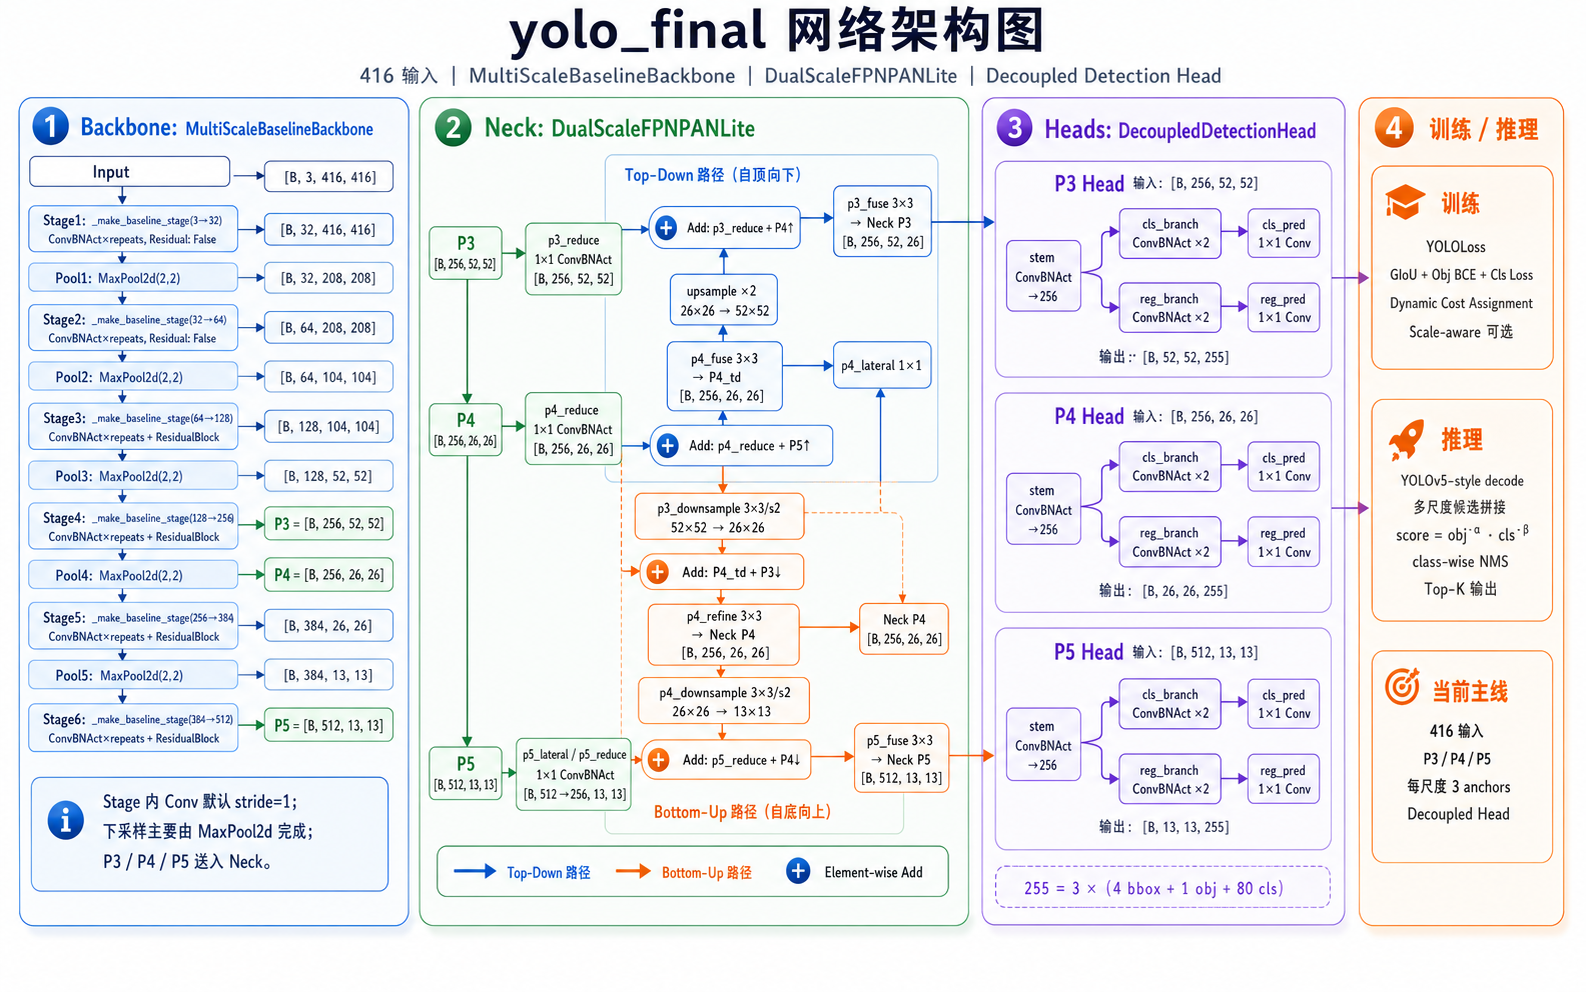
\includegraphics[width=\figwidth]{fbf6a2b881ca96ff418daff491125795.png}
  \caption{\code{yolo\_final} 网络架构示意图}
\end{figure}

\code{yolo\_final} 当前主线是一个 YOLO-style dense detector。整体流程可以概括为：

\[
  I \rightarrow B(I) \rightarrow N(P_4,P_5)
  \rightarrow H_4,H_5 \rightarrow \hat{Y}.
\]

其中，$I$ 表示输入图像，$B(\cdot)$ 表示 backbone，$N(\cdot)$ 表示 neck，$H_4,H_5$ 分别表示 P4 和 P5 上的检测头，$\hat{Y}$ 表示多尺度 prediction tensors。

从工程实现上看，模型由四个核心部分组成：

\begin{itemize}
  \item Backbone：将输入图像转换为不同空间分辨率和不同语义层级的特征图；
  \item Neck：使用轻量 FPN/PAN 路径融合 P4/P5 特征；
  \item Decoupled Head：每个尺度独立输出 box、objectness 和 class logits；
  \item Loss/Decoder：训练阶段进入 \code{YOLOLoss}，推理阶段进入 decode、score filtering 和 NMS。
\end{itemize}

当前模型输出两个尺度的 prediction tensors：

\[
  \hat{Y}_{p4} \in \mathbb{R}^{B \times 26 \times 26 \times 255},
  \quad
  \hat{Y}_{p5} \in \mathbb{R}^{B \times 13 \times 13 \times 255}.
\]

这里 $255 = 3 \times (4 + 1 + 80)$。其中 3 表示每个 grid cell 有 3 个 anchor；4 表示 box 参数；1 表示 objectness；80 表示 COCO 的类别 logits。

\begin{table}[h]
\centering
\caption{整体网络的张量接口}
\begin{tabular}{llll}
\toprule
模块 & 输入 & 输出 & 作用 \\
\midrule
Backbone & $[B,3,416,416]$ & $P_4,P_5$ & 提取多尺度视觉特征 \\
Neck & $P_4,P_5$ & $\tilde{P}_4,\tilde{P}_5$ & 融合语义与定位信息 \\
Head-P4 & $[B,C_4,26,26]$ & $[B,26,26,255]$ & 中等尺度目标预测 \\
Head-P5 & $[B,C_5,13,13]$ & $[B,13,13,255]$ & 大目标与强语义目标预测 \\
Decoder & 多尺度 logits & box/score/class & 生成检测结果 \\
\bottomrule
\end{tabular}
\end{table}

\section{Backbone 结构}

\begin{figure}[H]
  \centering
  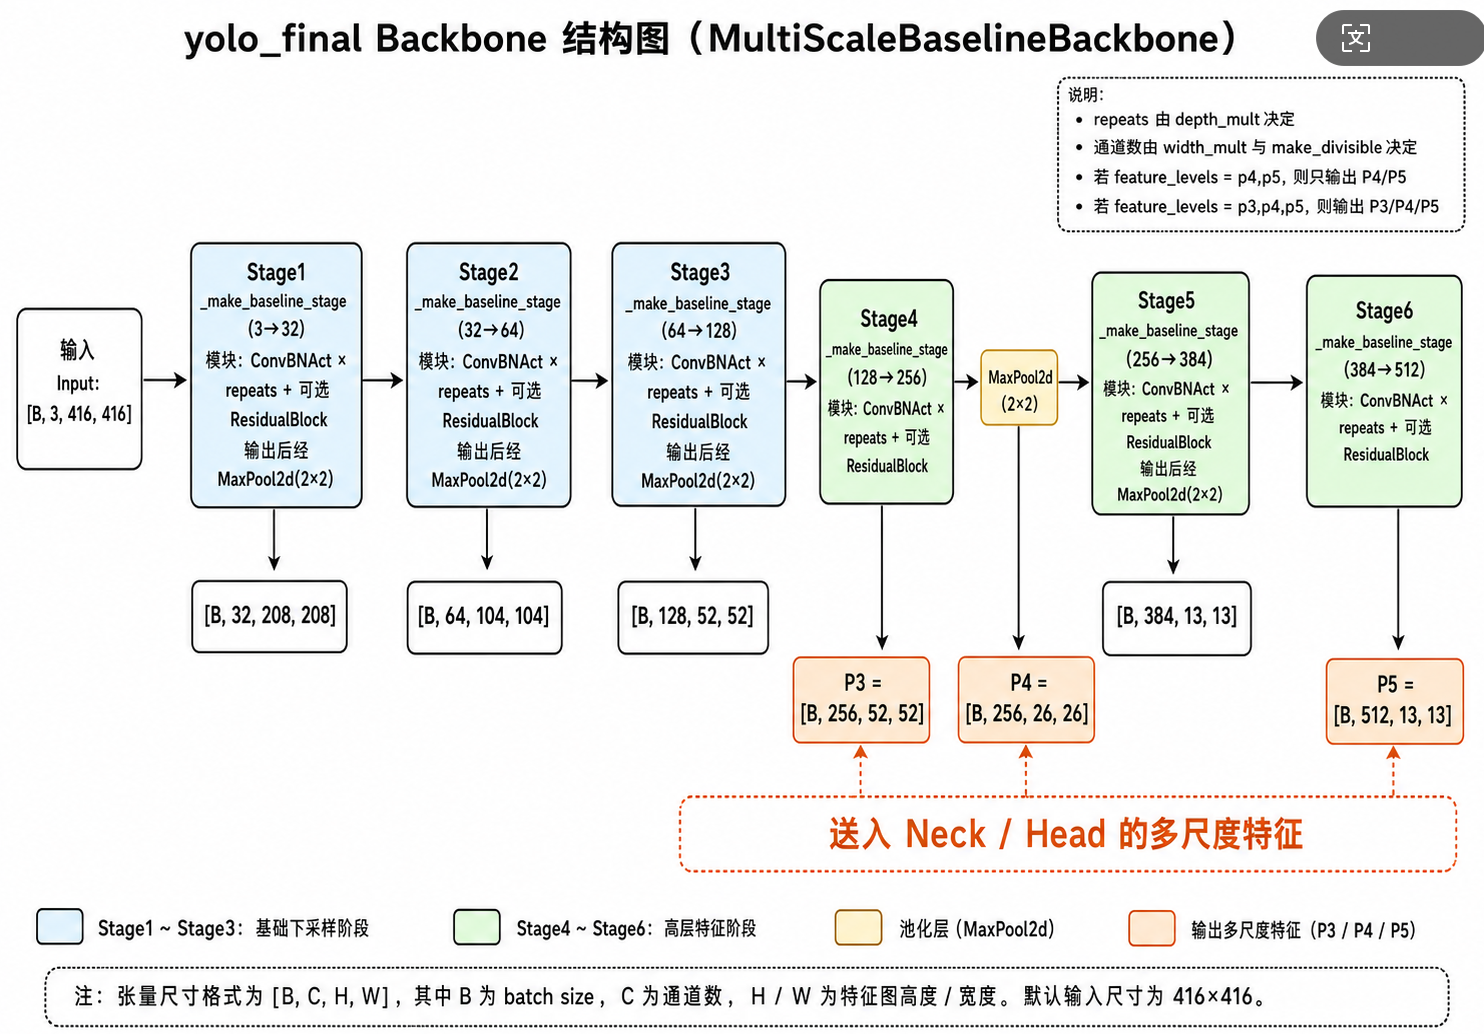
\includegraphics[width=\figwidth]{91292d3f0fa0b5cb851f90c19486d461.png}
  \caption{Backbone 结构示意图}
\end{figure}

当前主线使用的 backbone 是 \code{MultiScaleBaselineBackbone}。它由 6 个 stage 组成，通过卷积模块提取特征，并通过 MaxPool 完成空间下采样。前两个 stage 不使用残差模块，主要负责浅层纹理、边缘和局部组合模式的提取；从 stage3 开始加入 \code{ResidualBlock}，用于提升中后层表达能力并改善深层训练稳定性。

当输入图像尺寸为 $416 \times 416$ 时，当前主线主要使用两个检测尺度：

\begin{itemize}
  \item $P_4$：约 $26 \times 26$，通道数为 256，主要负责中等尺度目标；
  \item $P_5$：约 $13 \times 13$，通道数为 512，主要负责更大目标和更强语义目标。
\end{itemize}

在后续 P3 扩展实验中，模型会额外输出 $52 \times 52$ 的 P3 特征，用于增强小目标召回。但当前汇报的主线结构仍以 P4/P5 双尺度为核心。

\begin{table}[h]
\centering
\caption{Backbone stage 设计}
\begin{tabular}{llll}
\toprule
Stage & 通道数 & 是否 residual & 作用说明 \\
\midrule
Stage1 & 32 & 否 & 提取浅层纹理，随后下采样 \\
Stage2 & 64 & 否 & 提取边缘和局部组合模式 \\
Stage3 & 128 & 是 & 开始引入残差增强 \\
Stage4 & 256 & 是 & 产生 P3 候选特征，当前主线经 pool 得到 P4 \\
Stage5 & 384 & 是 & 聚合更强上下文语义 \\
Stage6 & 512 & 是 & 产生 P5 高语义特征 \\
\bottomrule
\end{tabular}
\end{table}

当前配置中 \code{depth\_mult=2.0}。每个 stage 内部基础卷积重复数为：

\[
  \mathrm{repeat}=\max(1,\mathrm{round}(2 \times \mathrm{depth\_mult}))=4.
\]

因此，每个 stage 不是单层卷积，而是由多层 \code{ConvBNAct} 加可选 \code{ResidualBlock} 构成。

\section{Backbone 小模块示意图}

\begin{figure}[H]
  \centering
  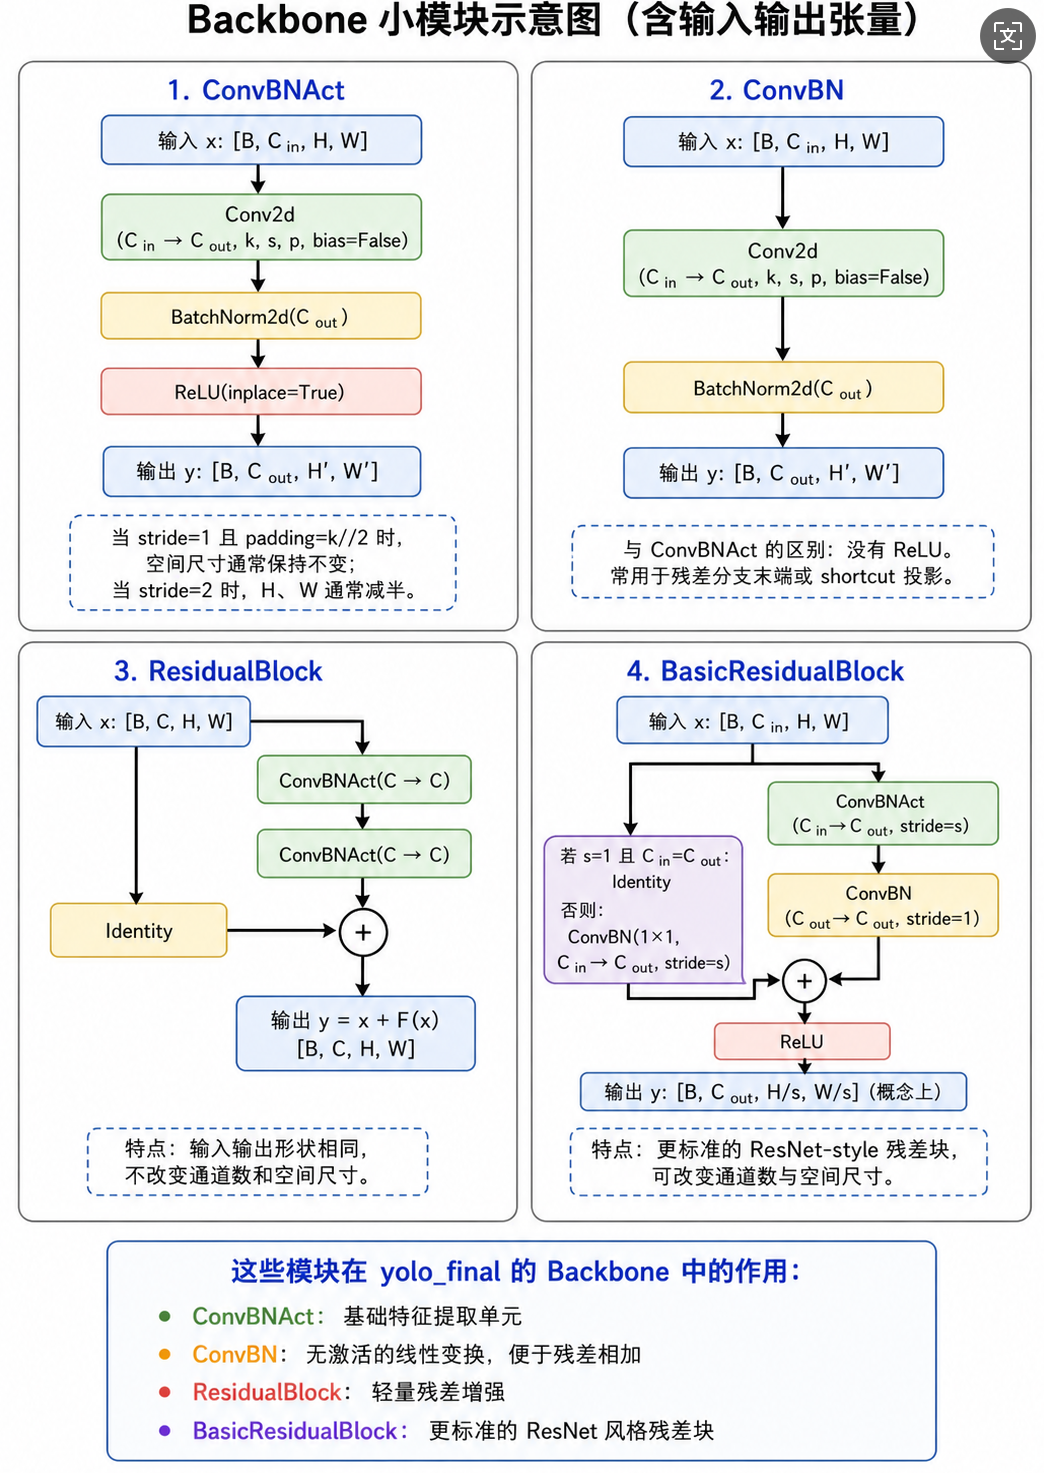
\includegraphics[width=\figwidth]{d445ecb7b5df8d9ab34431004f891f10.png}
  \caption{Backbone 小模块示意图}
\end{figure}

Backbone 中主要涉及三个基础模块：\code{ConvBNAct}、\code{ConvBN} 和 \code{ResidualBlock}。代码中也保留了 \code{BasicResidualBlock}，但当前主线没有使用 ResNet18-like backbone，因此它不是当前实验线的实际主干模块。

\subsection{ConvBNAct}

\code{ConvBNAct} 是最基础的特征提取模块，结构为：

\[
  \mathrm{Conv2d} \rightarrow \mathrm{BatchNorm2d} \rightarrow \mathrm{ReLU}.
\]

该模块负责局部感受野建模、通道变换和非线性表达，是 backbone、neck 和 head 中最常用的基础单元。

\subsection{ConvBN}

\code{ConvBN} 的结构为：

\[
  \mathrm{Conv2d} \rightarrow \mathrm{BatchNorm2d}.
\]

它不带激活函数，主要用于残差分支末端或 shortcut 对齐。保留无激活输出可以避免在残差相加前破坏线性残差路径。

\subsection{ResidualBlock}

当前主线实际使用的是轻量 \code{ResidualBlock}：

\[
  F(x)=\mathrm{ConvBNAct}_{3\times3}
  \left(\mathrm{ConvBNAct}_{3\times3}(x)\right),
  \quad
  y=x+F(x).
\]

该模块要求输入输出通道一致，不负责下采样，主要作用是在同一空间尺度上进一步细化特征。它可以缓解深层堆叠带来的优化难度，使中后层特征学习更加稳定。

\subsection{BasicResidualBlock}

\code{BasicResidualBlock} 是代码中保留的 ResNet 风格模块，支持 stride 下采样和 shortcut 通道对齐：

\[
  y=\mathrm{ReLU}(F(x)+S(x)).
\]

需要强调的是：当前实验线并不是没有残差块。从 stage3 到 stage6 都启用了 \code{ResidualBlock}；只是当前主线没有使用标准 ResNet 的 \code{BasicResidualBlock} 作为 backbone。

\section{检测器整体结构}

\begin{figure}[H]
  \centering
  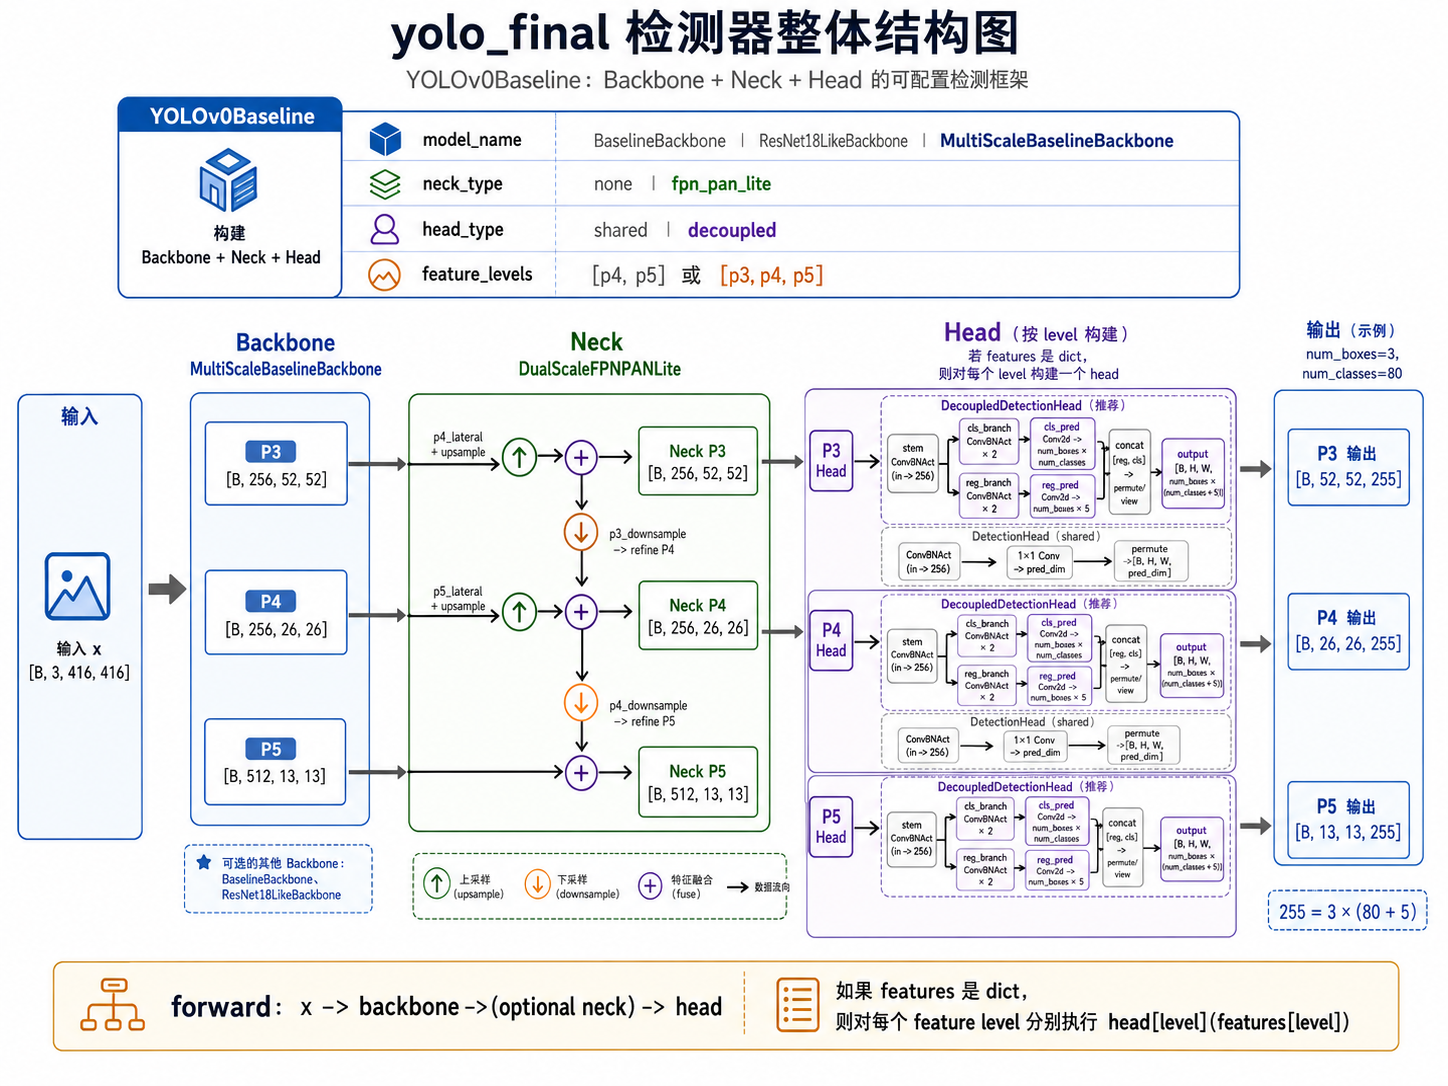
\includegraphics[width=\figwidth]{b325224c7d624b7fdb7fc89e19ba1d42.png}
  \caption{\code{yolo\_final} 检测器整体结构}
\end{figure}

检测器由 \code{YOLOv0Baseline} 作为统一入口进行构建。该类不是单一固定网络，而是根据配置动态组装 backbone、neck 和 head：

\begin{itemize}
  \item \code{\_build\_backbone}：根据 \code{model.name} 选择 backbone；
  \item \code{\_build\_neck}：根据 \code{neck\_type} 决定是否插入 FPN/PAN Lite；
  \item \code{\_build\_head}：根据 \code{head\_type} 选择 shared head 或 decoupled head。
\end{itemize}

当前主线中，backbone 和 neck 输出的是一个多尺度字典：

\[
  \{\code{p4}: \tilde{P}_4,\ \code{p5}: \tilde{P}_5\}.
\]

head 使用 \code{ModuleDict}，对每个尺度单独建立检测头，最终输出：

\[
  \{\code{p4}: \hat{Y}_{p4},\ \code{p5}: \hat{Y}_{p5}\}.
\]

\subsection{Neck：轻量 FPN/PAN 融合}

当前 neck 为 \code{DualScaleFPNPANLite}。它的作用是让 P4 获得更强的高层语义，同时让 P5 补充更细的定位信息。

Top-down 路径中，P5 经过 $1\times1$ lateral projection 后上采样，与 P4 对齐相加，再经过 $3\times3$ 卷积融合：

\[
  P_4^{td}=
  \mathrm{Conv}_{3\times3}
  \left(
  \mathrm{Conv}_{1\times1}(P_4)
  +
  \mathrm{Up}(\mathrm{Conv}_{1\times1}(P_5))
  \right).
\]

Bottom-up 路径中，融合后的 P4 再下采样回 P5 尺度，与原始 P5 投影结果相加：

\[
  P_5^{out}=
  \mathrm{Conv}_{3\times3}
  \left(
  \mathrm{Conv}_{1\times1}(P_5)
  +
  \mathrm{Down}(P_4^{out})
  \right).
\]

相对完整 FPN/PAN，当前版本更轻量，适合在我们当前 YOLOv1 实验框架中做可控对比。

\section{Decoupled Head 的结构介绍}

\begin{figure}[H]
  \centering
  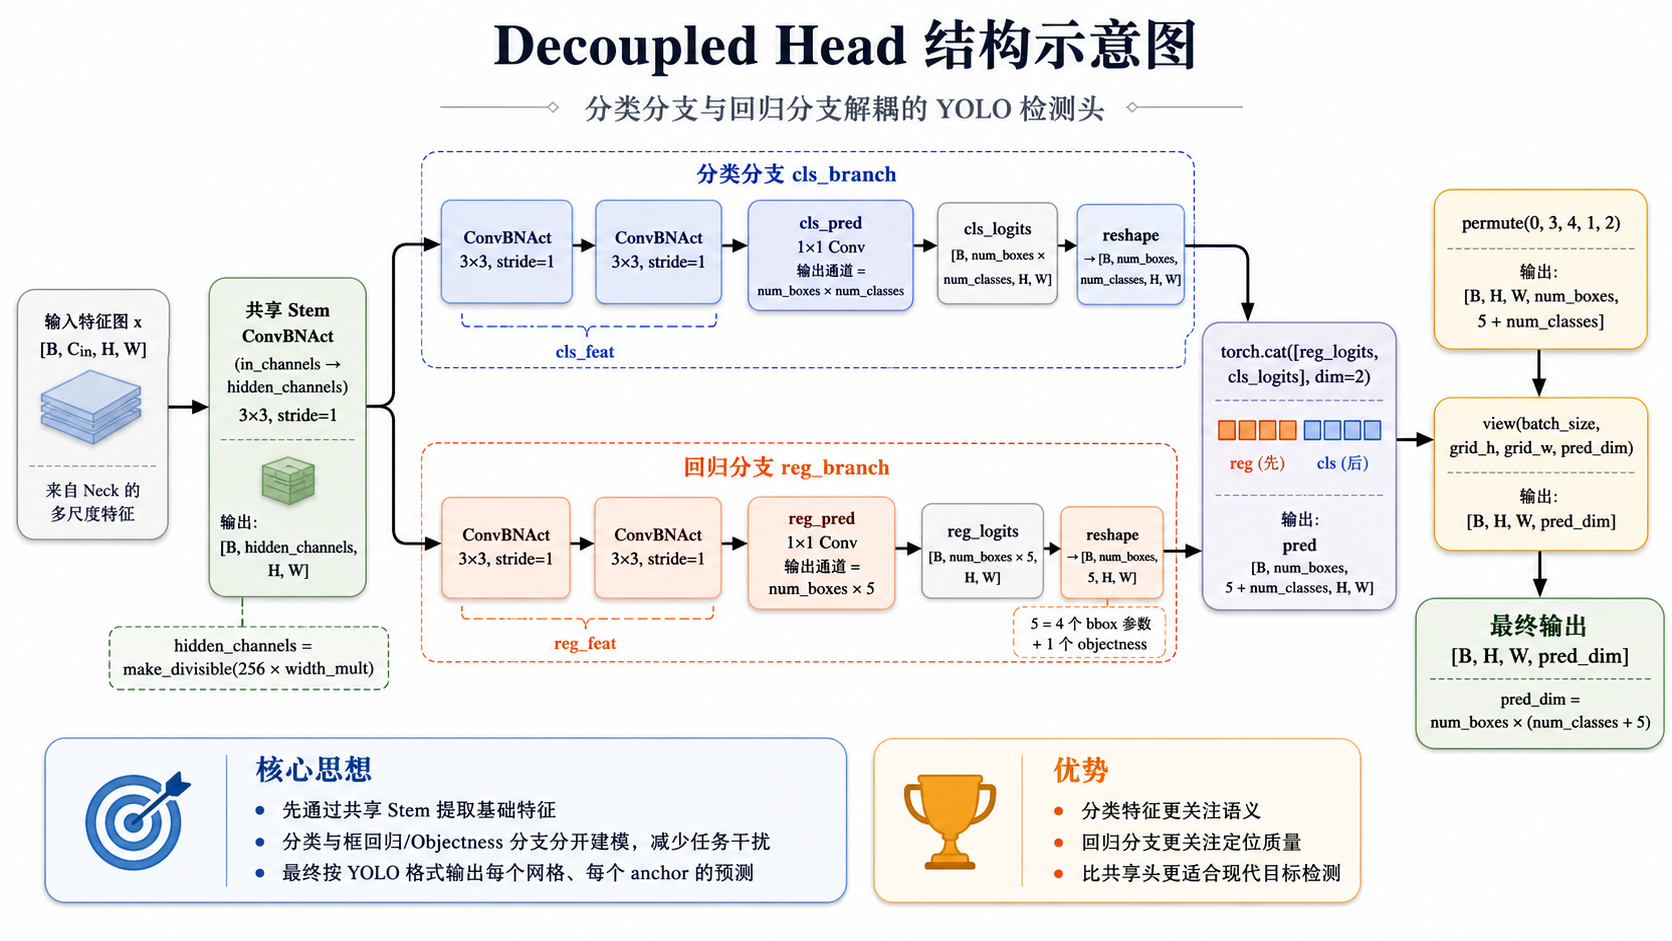
\includegraphics[width=\figwidth]{53d966dd7763d8002bbf99f1aed0445b.png}
  \caption{Decoupled Detection Head 结构示意图}
\end{figure}

当前主线检测头为 \code{DecoupledDetectionHead}。其核心思想是：分类任务和定位任务虽然共享输入特征，但在最后的预测分支中分开建模。

对任一尺度 $s$，输入特征为：

\[
  X_s \in \mathbb{R}^{B \times C_s \times H_s \times W_s}.
\]

首先经过 shared stem：

\[
  X_s' = \mathrm{ConvBNAct}_{3\times3}(X_s).
\]

然后进入两个独立分支：

\[
  Z_s^{cls} =
  \mathrm{Conv}_{1\times1}
  \left(\mathrm{ClsBranch}(X_s')\right)
  \in \mathbb{R}^{B \times (A C) \times H_s \times W_s},
\]

\[
  Z_s^{reg} =
  \mathrm{Conv}_{1\times1}
  \left(\mathrm{RegBranch}(X_s')\right)
  \in \mathbb{R}^{B \times (A \cdot 5) \times H_s \times W_s}.
\]

其中，classification branch 由两层 \code{ConvBNAct} 构成，输出 $A \times C$ 个类别 logits；regression branch 同样由两层 \code{ConvBNAct} 构成，输出 $A \times 5$ 个 box/objectness logits。

每个 anchor 的输出为：

\[
  (t_x,t_y,t_w,t_h,t_o,\ell_1,\ell_2,\ldots,\ell_{80}).
\]

最终 reshape 和 concat 后得到：

\[
  \hat{Y}_s \in \mathbb{R}^{B \times H_s \times W_s \times A(5+C)}.
\]

在当前 COCO 主线中，$A=3,C=80$，因此：

\[
  \hat{Y}_{p4} \in \mathbb{R}^{B \times 26 \times 26 \times 255},
  \quad
  \hat{Y}_{p5} \in \mathbb{R}^{B \times 13 \times 13 \times 255}.
\]

Decoupled head 的优势在于：分类更关注语义可分性，回归更关注几何定位和 objectness，两者不再完全共享最后的预测特征，有利于降低任务冲突。

\section{Prediction Tensors 到 Detection Results}

\begin{figure}[H]
  \centering
  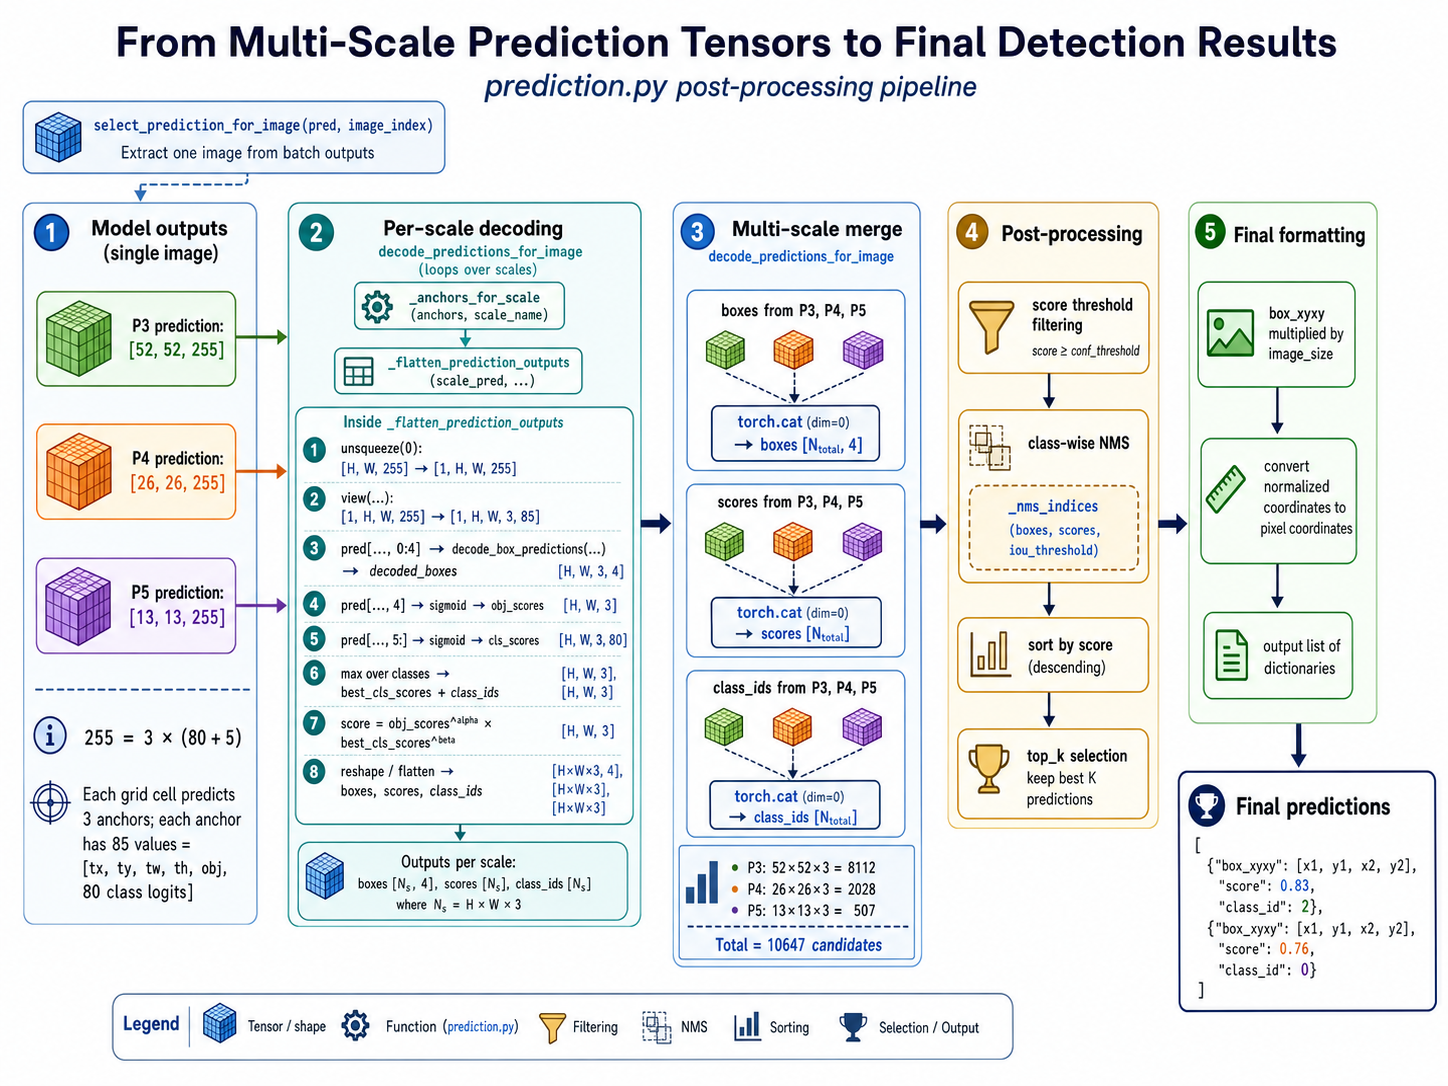
\includegraphics[width=\figwidth]{7cf3ea8aafb18db1c7bd66352c975a68.png}
  \caption{Prediction Tensors 到 Detection Results 的转换流程}
\end{figure}

推理阶段，模型输出的 prediction tensors 还不是最终检测结果。它们需要经过 decode、score 计算、阈值过滤和 NMS，才能转换为最终的 detection results。

整体流程如下：

\begin{enumerate}
  \item 按尺度取出 $\hat{Y}_{p4}$ 和 $\hat{Y}_{p5}$；
  \item 将每个尺度的输出 reshape 为 $[H,W,A,85]$；
  \item 根据 anchor 和 YOLOv5 box parameterization 解码 box；
  \item 对 objectness logit 和 class logits 做 sigmoid；
  \item 计算每个 anchor 的最终 score；
  \item 按 score threshold 过滤低置信度预测；
  \item 对每个类别执行 class-wise NMS；
  \item 按 score 降序排序并保留 top-k；
  \item 输出 box、score 和 class id。
\end{enumerate}

\subsection{Score 计算}

每个 anchor 的类别分数由 class logits 得到：

\[
  c^*=\arg\max_c \sigma(\ell_c),
  \quad
  p_{cls}=\max_c \sigma(\ell_c).
\]

最终排序分数为：

\[
  score=\sigma(t_o)^\alpha \cdot p_{cls}^\beta.
\]

当前评估和可视化中通常使用 $\alpha=2.0,\beta=1.0$，也就是说 objectness 被赋予更强的影响。如果 objectness 校准不好，最终排序会受到明显影响，因此我们后续也做过 score sweep 来检查 score calibration。

\subsection{最终检测结果格式}

最终每个 detection result 是一个字典：

\[
  \{\code{box\_xyxy},\ \code{score},\ \code{class\_id}\}.
\]

其中，\code{box\_xyxy} 表示左上角和右下角坐标。模型内部先在 resize 后的 $416 \times 416$ 坐标系中得到框；正式 COCO 评估时，会再映射回原始图像坐标。

\section{最终使用的 Loss 结构}

\begin{figure}[H]
  \centering
  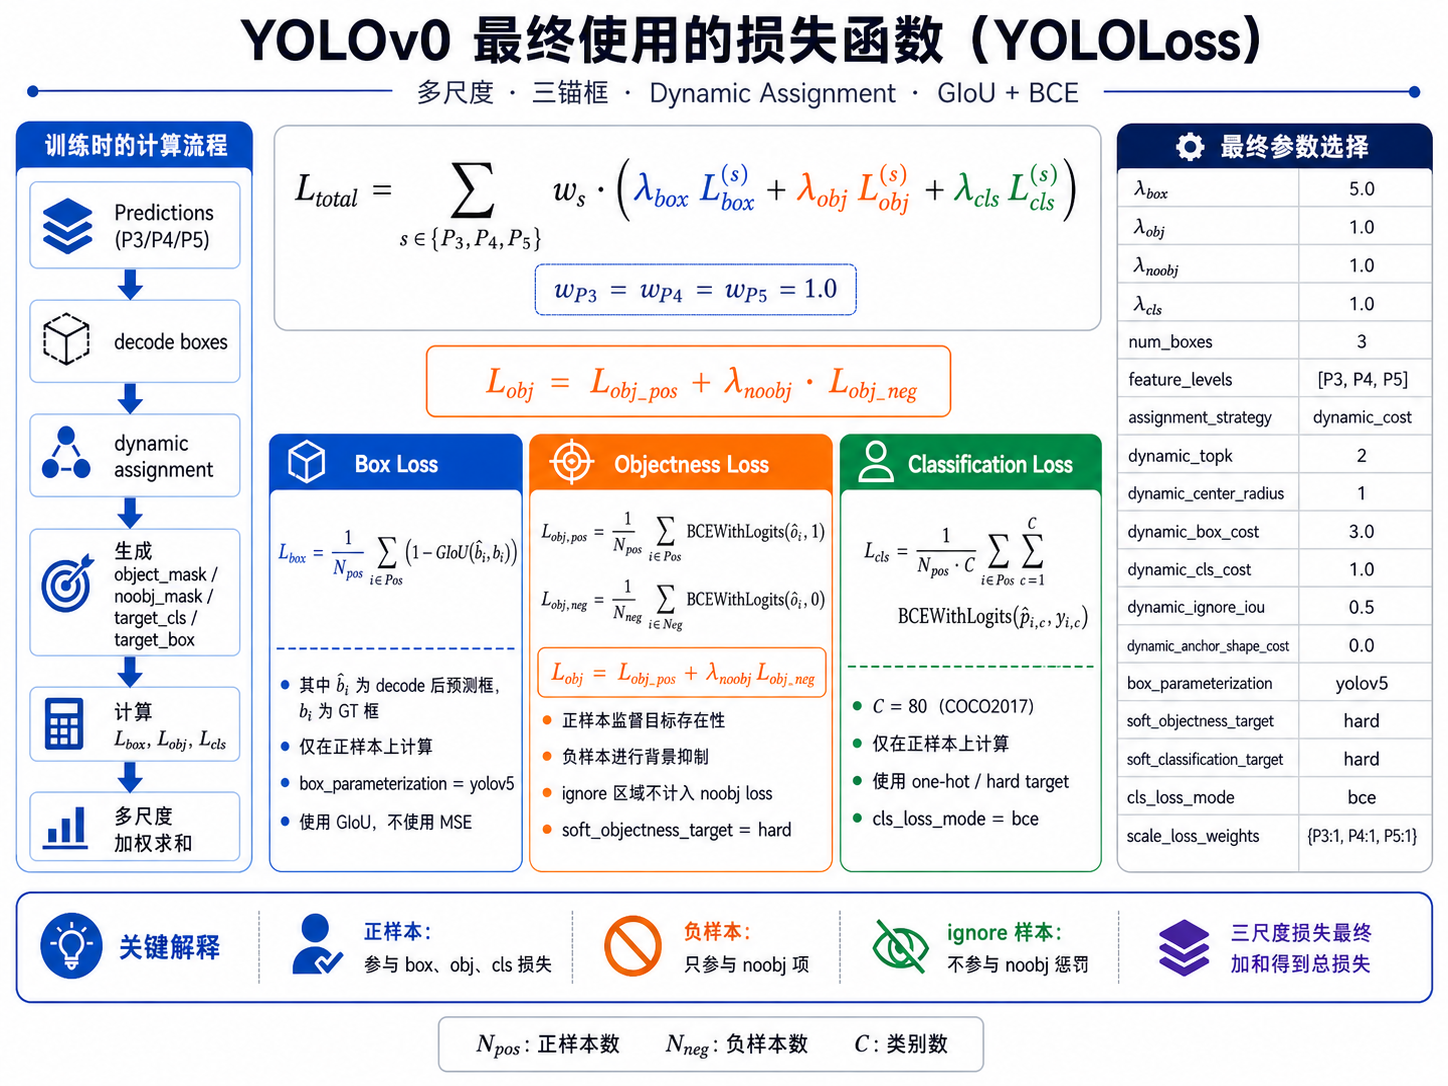
\includegraphics[width=\figwidth]{image.png}
  \caption{\code{YOLOLoss} 结构示意图}
\end{figure}

当前训练使用的 loss 由三个主要部分组成：box regression loss、objectness loss 和 classification loss。对于每个尺度 $s \in \{p4,p5\}$：

\[
  \mathcal{L}^{(s)}
  =
  \lambda_{box}\mathcal{L}_{box}^{(s)}
  +
  \lambda_{obj}\mathcal{L}_{obj}^{(s)}
  +
  \lambda_{cls}\mathcal{L}_{cls}^{(s)}.
\]

多尺度总 loss 为：

\[
  \mathcal{L}_{total}
  =
  \sum_s w_s\mathcal{L}^{(s)}.
\]

当前主线配置中：

\[
  \lambda_{box}=5,\quad
  \lambda_{obj}=1,\quad
  \lambda_{cls}=1,\quad
  \lambda_{noobj}=1.
\]

\subsection{Loss 前置步骤：Dynamic Assignment}

训练时，网络输出的是 dense predictions，即所有 grid cell、所有 anchor 上的预测槽位；而每张图中的 GT box 数量远少于预测槽位。因此，在计算 loss 之前，必须先决定每个 GT 由哪些预测槽位负责监督。

当前主线使用 \code{dynamic\_cost} assignment。对于每个 GT，先在 GT 中心附近选择候选 slots，然后计算匹配代价：

\[
  \mathrm{Cost}
  =
  \lambda_{box}^{cost}(1-\mathrm{IoU})
  +
  \lambda_{cls}^{cost}\mathrm{BCE}_{cls}
  +
  \lambda_{anchor}^{cost}\mathrm{ShapeCost}.
\]

其中：

\begin{itemize}
  \item $(1-\mathrm{IoU})$ 表示预测框与 GT 框的几何不匹配程度；
  \item $\mathrm{BCE}_{cls}$ 表示当前预测类别与 GT 类别之间的分类代价；
  \item $\mathrm{ShapeCost}$ 是可选 anchor shape prior，用于衡量 anchor 宽高与 GT 宽高的匹配程度；
  \item 主线基础配置中 $\lambda_{anchor}^{cost}=0$，后续 anchor-cost 实验中测试过非零形状先验。
\end{itemize}

每个 GT 根据 cost 选择最多 \code{dynamic\_topk=2} 个正样本。正样本参与 box loss、objectness positive loss 和 classification loss；负样本参与 objectness negative loss；高 IoU 但没有被分配为正样本的预测会被 ignore，不作为背景惩罚。

\subsection{Box Regression Loss}

Box regression loss 用于监督预测框的位置和尺度。当前使用 GIoU 形式：

\[
  \mathcal{L}_{box}
  =
  \frac{1}{N_{pos}}
  \sum_{i\in Pos}
  \left(1-\mathrm{GIoU}(b_i,\hat{b}_i)\right).
\]

其中，$N_{pos}$ 表示正样本数量，$b_i$ 表示预测框，$\hat{b}_i$ 表示对应 GT 框。

该项的物理意义是：让预测框与 GT 框在空间上尽可能重合。IoU 衡量预测框与 GT 框的重叠比例；GIoU 在两个框不相交时仍然能提供有效惩罚，因此比普通 IoU loss 更适合训练早期的框回归。

该 loss 只在 positive samples 上计算，不惩罚背景位置的 box。当前 $\lambda_{box}=5$，说明定位质量是总 loss 中权重最高的监督项。

\subsection{Objectness Loss}

Objectness loss 用于判断某个预测槽位是否负责一个真实目标。当前 objectness 被拆成正样本项和负样本项。

对正样本，objectness target 使用 IoU soft target：

\[
  y_{obj}^{+}
  =
  \max(\mathrm{IoU}(b_i,\hat{b}_i),\tau),
  \quad \tau=0.05.
\]

对应 loss 为：

\[
  \mathcal{L}_{obj}^{+}
  =
  \frac{1}{N_{pos}}
  \sum_{i\in Pos}
  \mathrm{BCEWithLogits}(o_i,y_{obj}^{+}).
\]

这里使用 IoU soft target 的原因是：objectness 不只表示“这里有没有目标”，也隐含表示“这个预测框是否高质量”。如果一个正样本框与 GT 的 IoU 很低，它不应该被训练成过高的 objectness。

对负样本，target 为 0：

\[
  \mathcal{L}_{obj}^{-}
  =
  \frac{1}{N_{neg}}
  \sum_{i\in Neg}
  \mathrm{BCEWithLogits}(o_i,0).
\]

最终 objectness loss 为：

\[
  \mathcal{L}_{obj}
  =
  \mathcal{L}_{obj}^{+}
  +
  \lambda_{noobj}\mathcal{L}_{obj}^{-}.
\]

我们将 $\lambda_{noobj}$ 从早期的 0.5 调整到 1.0，目的是增强背景抑制，降低误检候选框过多的问题。

\subsection{Classification Loss}

当前分类分支使用 \code{quality\_bce} 语义。分类目标不是简单 one-hot，而是质量感知 soft target：

\[
  y_{cls,c}
  =
  \begin{cases}
    \mathrm{IoU}(b_i,\hat{b}_i), & c=c^*,\\
    0, & c\neq c^*.
  \end{cases}
\]

分类 loss 为：

\[
  \mathcal{L}_{cls}
  =
  \frac{1}{N_{pos}C}
  \sum_{i\in Pos}\sum_{c=1}^{C}
  \mathrm{BCEWithLogits}(\ell_{i,c},y_{cls,c}).
\]

该项的意义是：分类置信度不仅表示目标属于哪个类别，还受到定位质量约束。低 IoU 的匹配不会被强行训练成高分类置信度，有助于让分类分数和框质量更一致。

\subsection{Loss 监控指标}

训练过程中除了记录总 loss，还需要记录各个子项和 assignment 指标。它们用于判断训练是否正常，但不等价于最终 COCO AP。

\begin{longtable}{lll}
\caption{Loss 相关监控指标}\\
\toprule
指标 & 含义 & 用途 \\
\midrule
\endfirsthead
\toprule
指标 & 含义 & 用途 \\
\midrule
\endhead
\code{loss\_box} & GIoU 框回归损失 & 判断定位学习是否改善 \\
\code{loss\_obj} & objectness 总损失 & 判断前景/背景置信度学习情况 \\
\code{loss\_obj\_pos} & 正样本 objectness loss & 看正样本置信度是否学起 \\
\code{loss\_obj\_neg} & 负样本 objectness loss & 看背景抑制是否足够 \\
\code{loss\_cls} & 分类 BCE loss & 判断类别分支学习情况 \\
\code{mean\_giou} & 正样本平均 GIoU & 定位质量的训练侧指标 \\
\code{mean\_obj\_target} & 正样本 objectness target 均值 & 检查 IoU soft target 状态 \\
\code{mean\_cls\_target} & 分类 soft target 均值 & 检查 quality target 状态 \\
\code{positive\_cells\_per\_image} & 每图正样本槽位数 & 检查 assignment 是否异常 \\
\code{collision\_count} & GT 落入同一 cell 的冲突数 & 检查 dense assignment 压力 \\
\code{ignored\_count} & ignore 槽位数 & 检查高 IoU 非正样本过滤情况 \\
\code{dropped\_gt\_count} & 未分配 GT 数 & 检查 GT 是否被漏分配 \\
\bottomrule
\end{longtable}

\section{本部分小结}

\code{yolo\_final} 当前主线是一个配置驱动的 YOLO-style dense detector，其结构可以概括为：

\[
  \mathrm{Backbone}
  +
  \mathrm{FPN/PAN\ Lite}
  +
  \mathrm{Decoupled\ MultiScale\ Heads}
  +
  \mathrm{YOLOLoss/Decoder}.
\]

当前模型的关键特点包括：

\begin{itemize}
  \item 使用 P4/P5 双尺度，兼顾中等目标和大目标；
  \item 每尺度 3 anchors；不同实验可使用原始 anchors 或 COCO train GT box 重新聚类 anchors；
  \item backbone 中实际使用残差结构，但不是标准 ResNet backbone；
  \item 使用 decoupled head，降低分类任务和定位任务在最终预测层的冲突；
  \item 使用 GIoU box loss、objectness BCE 和 quality-aware classification BCE；
  \item 训练侧通过 dynamic assignment 生成正负样本，推理侧通过 decode、score filtering 和 class-wise NMS 生成最终检测结果。
\end{itemize}

后续实验中的提高分辨率、重新聚类 anchors、增加 P3、调整 assignment 和 score calibration，本质上都围绕三个问题展开：特征尺度是否覆盖足够、候选框质量是否稳定、最终分数排序是否可靠。

\newpage

\section{第二部分：一次完整实验的流程与结果}

本部分选取实验
\[
\code{dual\_scale\_three\_box\_coco\_only\_noobj1\_416\_ddp\_20260430\_124818}
\]
作为完整案例，说明一次正式实验从配置、训练、保存、可视化、评估到指标解释的全流程。该实验是 COCO-only、P4/P5 双尺度、每尺度 3 anchor、原始 P4/P5 anchor、$\lambda_{noobj}=1.0$ 的 8 GPU DDP 训练实验，也是当前正式 COCO AP、AP50、AP75 综合最好的结果展示轮次。

\subsection{实验结果展示}

训练脚本在实验结束后默认保存 4 张验证集可视化结果。这 4 张图主要用于快速 sanity check：观察模型是否能输出框、类别是否大致合理、置信度是否过低或过高、是否存在明显候选框爆炸。

\begin{figure}[H]
\centering
\begin{minipage}{0.48\textwidth}
\centering

\includegraphics[width=\linewidth]{../../outputs/dual_scale_three_box_coco_only_noobj1_416_ddp_20260430_124818/visualizations/coco2017_val_000000037777.png}
\end{minipage}
\hfill
\begin{minipage}{0.48\textwidth}
\centering

\includegraphics[width=\linewidth]{../../outputs/dual_scale_three_box_coco_only_noobj1_416_ddp_20260430_124818/visualizations/coco2017_val_000000087038.png}
\end{minipage}

\vspace{0.5em}

\begin{minipage}{0.48\textwidth}
\centering

\includegraphics[width=\linewidth]{../../outputs/dual_scale_three_box_coco_only_noobj1_416_ddp_20260430_124818/visualizations/coco2017_val_000000252219.png}
\end{minipage}
\hfill
\begin{minipage}{0.48\textwidth}
\centering

\includegraphics[width=\linewidth]{../../outputs/dual_scale_three_box_coco_only_noobj1_416_ddp_20260430_124818/visualizations/coco2017_val_000000397133.png}
\end{minipage}
\caption{本轮实验默认保存的 4 张验证集检测可视化}
\end{figure}

为了最终汇报，我们额外保存 12 张扩展展示图作为更完整的结果展示。该组图与上面的 4 张图使用同一套展示参数：score threshold 0.25、top-k 12、score $\alpha=2.0,\beta=1.0$。这样不同展示图之间的框数量和置信度筛选规则保持一致，便于直接比较视觉效果。

\begin{figure}[H]
\centering
\begin{minipage}{0.23\textwidth}
\includegraphics[width=\linewidth]{../../outputs/evaluations/dual_scale_three_box_coco_only_noobj1_416_ddp_20260430_124818_display_vis12/coco2017_val_000000006818.png}\end{minipage}\hfill
\begin{minipage}{0.23\textwidth}
\includegraphics[width=\linewidth]{../../outputs/evaluations/dual_scale_three_box_coco_only_noobj1_416_ddp_20260430_124818_display_vis12/coco2017_val_000000037777.png}\end{minipage}\hfill
\begin{minipage}{0.23\textwidth}
\includegraphics[width=\linewidth]{../../outputs/evaluations/dual_scale_three_box_coco_only_noobj1_416_ddp_20260430_124818_display_vis12/coco2017_val_000000087038.png}\end{minipage}\hfill
\begin{minipage}{0.23\textwidth}
\includegraphics[width=\linewidth]{../../outputs/evaluations/dual_scale_three_box_coco_only_noobj1_416_ddp_20260430_124818_display_vis12/coco2017_val_000000174482.png}\end{minipage}

\vspace{0.45em}

\begin{minipage}{0.23\textwidth}
\includegraphics[width=\linewidth]{../../outputs/evaluations/dual_scale_three_box_coco_only_noobj1_416_ddp_20260430_124818_display_vis12/coco2017_val_000000252219.png}\end{minipage}\hfill
\begin{minipage}{0.23\textwidth}
\includegraphics[width=\linewidth]{../../outputs/evaluations/dual_scale_three_box_coco_only_noobj1_416_ddp_20260430_124818_display_vis12/coco2017_val_000000296649.png}\end{minipage}\hfill
\begin{minipage}{0.23\textwidth}
\includegraphics[width=\linewidth]{../../outputs/evaluations/dual_scale_three_box_coco_only_noobj1_416_ddp_20260430_124818_display_vis12/coco2017_val_000000331352.png}\end{minipage}\hfill
\begin{minipage}{0.23\textwidth}
\includegraphics[width=\linewidth]{../../outputs/evaluations/dual_scale_three_box_coco_only_noobj1_416_ddp_20260430_124818_display_vis12/coco2017_val_000000386912.png}\end{minipage}

\vspace{0.45em}

\begin{minipage}{0.23\textwidth}
\includegraphics[width=\linewidth]{../../outputs/evaluations/dual_scale_three_box_coco_only_noobj1_416_ddp_20260430_124818_display_vis12/coco2017_val_000000397133.png}\end{minipage}\hfill
\begin{minipage}{0.23\textwidth}
\includegraphics[width=\linewidth]{../../outputs/evaluations/dual_scale_three_box_coco_only_noobj1_416_ddp_20260430_124818_display_vis12/coco2017_val_000000403385.png}\end{minipage}\hfill
\begin{minipage}{0.23\textwidth}
\includegraphics[width=\linewidth]{../../outputs/evaluations/dual_scale_three_box_coco_only_noobj1_416_ddp_20260430_124818_display_vis12/coco2017_val_000000458054.png}\end{minipage}\hfill
\begin{minipage}{0.23\textwidth}
\includegraphics[width=\linewidth]{../../outputs/evaluations/dual_scale_three_box_coco_only_noobj1_416_ddp_20260430_124818_display_vis12/coco2017_val_000000480985.png}\end{minipage}
\caption{本轮实验用于最终展示的 12 张扩展展示图}
\end{figure}

\subsection{实验流程与配置文件}

该实验使用的配置文件快照为：
\[
\code{logs/records/dual\_scale\_three\_box\_coco\_only\_noobj1\_416\_ddp\_20260430\_124818/config.toml}.
\]
原始配置来自：
\[
\code{configs/dual\_scale\_three\_box\_coco\_only\_noobj1\_416.toml}.
\]

\begin{table}[H]
\centering
\caption{本轮实验的关键配置}
\begin{tabular}{ll}
\toprule
类别 & 配置 \\
\midrule
训练集 & COCO2017 train，118287 张 \\
验证集 & COCO2017 val，5000 张 \\
数据格式 & packed \code{.pt}，chunk size 1024，cache 4 chunks \\
输入尺寸 & $416 \times 416$ \\
数据增广 & 本轮无随机增广；执行 resize 与 box 同步缩放 \\
模型 & P4/P5 双尺度，decoupled head，FPN/PAN Lite \\
Anchor & 原始 P4/P5 anchors \\
Loss & GIoU + objectness BCE + quality-aware cls BCE \\
Assignment & \code{dynamic\_cost}，\code{dynamic\_topk=2} \\
优化器 & AdamW，lr 0.001，weight decay 0.0001 \\
学习率调度 & cosine，min lr $1\times10^{-5}$ \\
训练轮数 & 30 epoch \\
并行方式 & 8 GPU DDP，NCCL backend \\
Batch size & 每卡 16，全局有效 batch size 128 \\
DataLoader & 总 \code{num\_workers=64}，每 rank 8 workers \\
\bottomrule
\end{tabular}
\end{table}

训练流程可以概括为：先读取配置文件并构建 COCO-only dataset；随后校验 packed \code{.pt} index 与 chunk 文件是否完整；再构建 P4/P5 双尺度模型、原始 P4/P5 anchors、\code{YOLOLoss}、AdamW optimizer 和 cosine scheduler；最后通过 \code{torchrun} 启动 8 进程 DDP 训练。每个 epoch 后进行 validation，并按 best validation loss 保存 \code{best.pth}。

本轮训练从零开始，没有从已有 checkpoint resume。实验完成状态为 \code{completed}。训练总耗时约 24117.2 秒，验证总耗时约 665.4 秒，训练加验证合计约 6.884 小时。单个训练 epoch 平均约 803.9 秒，即约 13.40 分钟；单个 validation epoch 平均约 22.2 秒。每个 epoch 有 925 个 optimizer steps，训练全量样本约 118288，验证样本为 5000。

\subsection{训练过程中保存的检测与监控指标}

本轮模型 profile 的正式记录来自 COCO eval JSON。训练过程中的 loss、learning rate、assignment 指标和定位质量指标以 TensorBoard event 为原始记录来源，对应目录为：
\[
\code{runs/dual\_scale\_three\_box\_coco\_only\_noobj1\_416\_ddp\_20260430\_124818}.
\]
模型参数量为 36.53M，总 FLOPs 为 78.38 GFLOPs。测速配置为 batch size 1，warmup 20 次，measure 100 次；记录到的平均推理耗时为 3.53 ms/batch，吞吐约 283.32 images/s。这里的 FLOPs 统计主要来自 Conv2d，Linear FLOPs 为 0。

\begin{figure}[H]
\centering
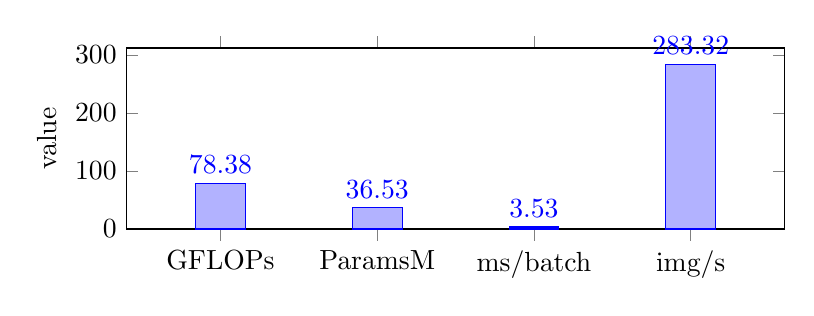
\begin{tikzpicture}
\begin{axis}[
  ybar,
  width=0.82\textwidth,
  height=0.32\textwidth,
  symbolic x coords={GFLOPs,ParamsM,ms/batch,img/s},
  xtick=data,
  ylabel={value},
  nodes near coords,
  nodes near coords align={vertical},
  ymin=0,
  bar width=18pt,
  enlarge x limits=0.2
]
\addplot coordinates {(GFLOPs,78.38) (ParamsM,36.53) (ms/batch,3.53) (img/s,283.32)};
\end{axis}
\end{tikzpicture}
\caption{本轮实验模型复杂度与推理 profile。不同柱子的单位不同，图中用于集中展示 profile 量级。}
\end{figure}

Loss 下降曲线如下。该图由 TensorBoard 中的 epoch 级标量导出，使用的 tag 包括 \code{loss/total\_epoch}、\code{val/total\_epoch}、\code{loss/box\_epoch} 和 \code{val/box\_epoch}。训练集 loss 从 7.2061 降到 3.7613，验证集 loss 从 6.8091 降到 4.8544；best validation loss 出现在第 23 轮，为 4.7799。训练 loss 持续下降，而验证 loss 在后期趋于平台并略有回升，说明模型已经进入明显的收敛后段。

\begin{figure}[H]
\centering
\begin{tikzpicture}
\begin{axis}[
  width=0.88\textwidth,
  height=0.43\textwidth,
  xlabel={epoch},
  ylabel={loss},
  grid=major,
  legend pos=north east
]
\addplot+[mark=none, thick] table[x=epoch,y=train_total] {best416_loss.dat};
\addlegendentry{train total}
\addplot+[mark=none, thick] table[x=epoch,y=val_total] {best416_loss.dat};
\addlegendentry{val total}
\addplot+[mark=none, dashed] table[x=epoch,y=train_box] {best416_loss.dat};
\addlegendentry{train box}
\addplot+[mark=none, dashed] table[x=epoch,y=val_box] {best416_loss.dat};
\addlegendentry{val box}
\end{axis}
\end{tikzpicture}
\caption{训练集与验证集 loss 下降曲线}
\end{figure}

TensorBoard 同时保存了 step 级训练标量。由于 DDP 中 step 级 TensorBoard 当前记录的是 rank0 局部 batch 的 loss，因此它更适合观察训练过程是否发散、是否存在异常尖峰，而不应被解释为 8 卡全局平均 step loss。下图使用 \code{rank0\_loss/*\_step} 标量下采样绘制，用于展示 step 级训练波动。

\begin{figure}[H]
\centering
\begin{tikzpicture}
\begin{axis}[
  width=0.88\textwidth,
  height=0.38\textwidth,
  xlabel={global step},
  ylabel={rank0 step loss},
  grid=major,
  legend pos=north east
]
\addplot+[mark=none, thick] table[x=step,y=total] {best416_tb_step_loss.dat};
\addlegendentry{total}
\addplot+[mark=none, dashed] table[x=step,y=box] {best416_tb_step_loss.dat};
\addlegendentry{box}
\addplot+[mark=none, dashed] table[x=step,y=obj] {best416_tb_step_loss.dat};
\addlegendentry{objectness}
\addplot+[mark=none, dotted] table[x=step,y=cls] {best416_tb_step_loss.dat};
\addlegendentry{classification}
\end{axis}
\end{tikzpicture}
\caption{TensorBoard step 级 rank0 loss 曲线。图中数据来自 \code{rank0\_loss/*\_step}，为版面展示做了下采样。}
\end{figure}

下面的图展示 epoch-to-epoch 的 loss 改变量。它同样由 TensorBoard epoch scalar 计算得到，用于监控 loss 下降速度，也就是“loss 曲线的一阶变化”。需要注意，这不是参数梯度范数；本轮实验没有保存真实的 parameter grad norm。因此该图只能说明 loss 收敛速度，而不能替代梯度范数监控。后续若要做真正的梯度监控，需要在训练脚本中额外记录 \code{grad\_norm}、是否出现 NaN/Inf、以及必要时的 gradient clipping 状态。

\begin{figure}[H]
\centering
\begin{tikzpicture}
\begin{axis}[
  width=0.88\textwidth,
  height=0.38\textwidth,
  xlabel={epoch},
  ylabel={previous loss - current loss},
  grid=major,
  legend pos=north east
]
\addplot+[mark=none, thick] table[x=epoch,y=train_improve] {best416_loss_delta.dat};
\addlegendentry{train loss decrease}
\addplot+[mark=none, thick] table[x=epoch,y=val_improve] {best416_loss_delta.dat};
\addlegendentry{val loss decrease}
\addplot+[mark=none, black, dashed] coordinates {(1,0) (30,0)};
\end{axis}
\end{tikzpicture}
\caption{Loss 下降速度监控。负值表示该 epoch 的 loss 相比上一轮上升。}
\end{figure}

除了 loss，本轮 TensorBoard 还记录了 assignment 与定位相关指标。正样本平均 GIoU 从训练第 1 轮的 0.4814 提升到第 30 轮的 0.7554；验证 mean GIoU 从 0.5179 提升到 0.6823。每图正样本槽位数约从 26--27 提升并稳定在 28 左右，说明 dynamic assignment 持续给每张图分配了稳定数量的正样本。

\begin{figure}[H]
\centering
\begin{tikzpicture}
\begin{axis}[
  width=0.88\textwidth,
  height=0.40\textwidth,
  xlabel={epoch},
  ylabel={value},
  grid=major,
  legend pos=south east
]
\addplot+[mark=none, thick] table[x=epoch,y=train_giou] {best416_monitor.dat};
\addlegendentry{train mean GIoU}
\addplot+[mark=none, thick] table[x=epoch,y=val_giou] {best416_monitor.dat};
\addlegendentry{val mean GIoU}
\addplot+[mark=none, dashed] table[x=epoch,y=train_dropped] {best416_monitor.dat};
\addlegendentry{train dropped GT}
\addplot+[mark=none, dashed] table[x=epoch,y=val_dropped] {best416_monitor.dat};
\addlegendentry{val dropped GT}
\end{axis}
\end{tikzpicture}
\caption{定位与 assignment 健康度监控}
\end{figure}

\subsection{正式 COCO 指标与实际意义}

COCO AP 使用多个 IoU 阈值综合评价检测质量。AP 是 $0.50:0.05:0.95$ 共 10 个 IoU 阈值上的平均 precision-recall 面积；AP50 只看 IoU=0.50，主要反映粗定位下的召回和分类能力；AP75 更强调较准确定位。APS、APM、APL 分别对应 small、medium、large 三种目标尺寸。AR1、AR10、AR100 表示每张图最多保留 1、10、100 个预测时的平均召回能力。

\begin{table}[H]
\centering
\caption{COCO 指标含义与本轮结果}
\begin{tabular}{lll}
\toprule
指标 & 计算规则/含义 & 本轮结果 \\
\midrule
AP & IoU 0.50:0.95 平均 AP & 0.1488 \\
AP50 & IoU=0.50 的 AP & 0.2487 \\
AP75 & IoU=0.75 的 AP & 0.1553 \\
AP small & 小目标 AP & 0.056 \\
AP medium & 中目标 AP & 0.159 \\
AP large & 大目标 AP & 0.214 \\
AR1 & 每图最多 1 个预测的平均召回 & 0.1889 \\
AR10 & 每图最多 10 个预测的平均召回 & 0.2898 \\
AR100 & 每图最多 100 个预测的平均召回 & 0.3023 \\
预测数量 & 全验证集最终预测框数 & 260274 \\
预测/图 & 平均每张图预测框数量 & 52.0548 \\
\bottomrule
\end{tabular}
\end{table}

\begin{figure}[H]
\centering
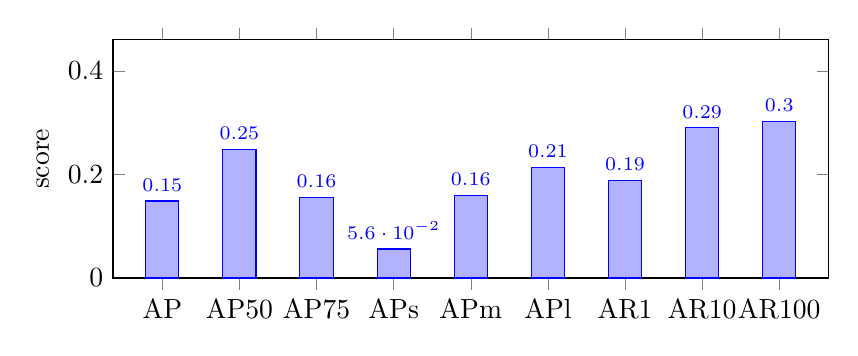
\begin{tikzpicture}
\begin{axis}[
  ybar,
  width=0.88\textwidth,
  height=0.38\textwidth,
  symbolic x coords={AP,AP50,AP75,APs,APm,APl,AR1,AR10,AR100},
  xtick=data,
  ymin=0,
  ymax=0.46,
  ylabel={score},
  nodes near coords,
  nodes near coords style={font=\scriptsize},
  bar width=12pt,
  enlarge x limits=0.08
]
\addplot coordinates {
  (AP,0.1488) (AP50,0.2487) (AP75,0.1553)
  (APs,0.0560) (APm,0.1590) (APl,0.2140)
  (AR1,0.1889) (AR10,0.2898) (AR100,0.3023)
};
\end{axis}
\end{tikzpicture}
\caption{本轮实验 COCO AP/AR 指标可视化}
\end{figure}

从结果解释上看，本轮模型已经具备基本检测能力，但距离成熟 YOLO 检测器仍有明显差距。AP50 高于 AP75，说明模型在“粗略找到目标”方面优于“高质量定位”；AP small 明显低于 AP medium 和 AP large，说明当前 P4/P5 双尺度结构对小目标不够友好，这也是后续增加 P3 的直接动机。AR100 为 0.3023，说明即便每张图允许保留较多候选，召回仍然有限，因此后续改进不能只靠降低 score threshold，还需要从分辨率、P3 特征、小目标 anchor 和 assignment 上继续提升候选质量。

本轮默认评估配置为 score threshold 0.05、top-k 100、NMS IoU 0.5、score $\alpha=2.0,\beta=1.0$。后续非训练 sweep 显示，在不重新训练的情况下，在 500 张诊断子集上，score threshold 0.01 可提升 AP 到约 0.1800，NMS IoU 0.7 可将 AR100 提高到约 0.3361。这说明当前模型仍有一部分召回受到推理阈值和 NMS 设置影响，但正式结论仍以全量 COCO eval 为准，根本改进仍需要训练方向的结构和数据策略调整。

\end{CJK*}
\end{document}
